\chapter{Návrh rozšíření Node-RED a komunikačního protokolu}
\label{ch:protokol}

V~této kapitole bude popsán princip funkce koncových uzlů a způsob, kterým s~nimi bude komunikováno.
S~využitím možností, které nabízí jazyk MicroPython, popsaných v~kapitole~\ref{sec:micropython}, jsem se rozhodl
koncové uzly používat víceúčelově -- v~jeden moment na uzlu může více instancí aplikací.
\textbf{Aplikace} je v~kontextu této práce jednoúčelový program ovládající konkrétní periferii uzlu -- pro svou činnost
využívá rozhraní poskytnutého operačním systémem běžícím na ESP32.
O~přepínání kontextu se stará operační systém, stejně jako o~připojení k~Internetu, brokeru MQTT a o~správu uzlu jako
takového.

Aplikace je možné dělit na vstupní (data z~reálného světa posílají pomocí zpráv do sítě) a na výstupní (data ze sítě
transformují na interakci s~okolním světem).

\section{Požadavky na protokol}\label{sec:pozadavky-na-protokol}
Základním spojovacím prvkem nástroje Node-RED a vlastních uzlů je rozhraní, pomocí kterého budou
komunikovat.
S~využitím protokolu MQTT a jeho vlastností popíšu v~této kapitole základní požadavky na komunikační protokol a
následně jej navrhnu -- ze základních požadavků poté budou plynout i požadavky na obě strany komunikace (uzly i
Node-RED -- centrální uzel).

Na základě povahy a potřeb obou komunikujících stran jsem navrhnul tyto základní požadavky:
\begin{enumerate}
    \item \textbf{Pro zprávy je použit formát JSON} \\
    Důvodem je jeho jednoduchost, kvalitní podpora a textová podstata (tedy i snažší ladění).
    Ze strany Node-RED je tento formát implicitní -- jedná se o~\uv{Javascript Object Notation} -- serializace a
    deserializace probíhají zcela přirozeně.
    Na straně uzlů pak poskytuje MicroPython kompletní podporu pro tento formát -- deserializace probíhá do
    vestavěných typů.

    \item \textbf{Samostatné kanály pro směry \uv{do uzlu} a \uv{z~uzlu}} \\
    Pro snížení datového toku a cílení zpráv pro konkrétní uzly je nutné oddělit komunikační kanály pro každý
    samostatný uzel -- rozšíření na straně Node-RED zajistí směřování do konkrétních kanálů dle konfigurace a uzly
    naopak odběr kanálů pouze příslušících danému uzlu.

    \item \textbf{Samostatné kanály pro jednotlivé aplikace na uzlu} \\
    Jednotlivé aplikace běžící na uzlech je nutné v~protokolu od sebe oddělovat -- tzn. kromě rozlišení na úrovni
    všech uzlů musí dojít k~rozlišení běžících aplikací na úrovni jednoho uzlu.

    \item \textbf{Obsah zprávy je plně v~režii aplikace} \\
    Protokol jako takový nevyžaduje \emph{(kromě vlastních režijních zpráv)} konkrétní obsah zpráv -- jejich schéma a
    datové typy obsahu jsou plně v~režii komunikující dvojice aplikace na uzlu a bloku v~nástroji Node-RED.

    \item \textbf{Kanály pro status a sběr běhových informací z~uzlu} \\
    Jedním z~požadovaných kanálů je zpětný kanál statusu uzlu, kterým bude uzel oznamovat do sítě svůj stav (připojen či
    nepřipojen), případně další informace (využití úložiště, čekající data).
    Další požadovaný kanál z~tohoto hlediska je kanál pro běhové informace z~uzlu -- logy, které budou obsahovat
    stručný popis stavu, ke kterému na uzlu došlo -- od vyjímkových stavů až k~čistě ladícím informacím.

    \item \textbf{Kanál pro konfiguraci uzlu} \\
    Pro režijní komunikaci s~uzlem je nutný samostatný konfigurační kanál, pomocí kterého bude uzel příjmat příkazy
    k~zavedení aplikace, její překonfigurování či ukončení -- dále pomocí něj mohou být přenášeny informace o~vytížení
    uzlu či nastavení připojení k~nástroji Node-RED, potažmo brokeru MQTT.
\end{enumerate}

\section{Kanály MQTT}\label{sec:mqtt-kanaly}
Na základě všech vlastností protokolu MQTT popsaných v~kapitole~\ref{sec:mqtt} jsem právě jej zvolil za spojovací
prvek koncových uzlů a uzlu centrálního (nástroje Node-RED).
V~popisu navržených kanálů budou použity následující symboly:
\begin{itemize}
    \item \ic{NODE_ID} je jednoznačná textová identifikace uzlu v~síti
    \item \ic{APP_ID} je jednoznačná textová identifikace instance aplikace v~rámci uzlu
    \item \ic{\#} je zástupný znak popsaný v~kapitole~\ref{sec:mqtt}
    \item \ic{fis} \textbf{je zkratka z~Fast IoT Solution -- programového názvu pro tuto práci}
\end{itemize}

Na základě požadavků stanovených v~kapitole~\ref{sec:pozadavky-na-protokol} jsem navrhnul použití následujících
kanálů MQTT (funkce budou popsány z~pohledu centrálního uzlu):

\begin{itemize}
    \item \ic{fis/to/NODE_ID/app/APP_ID} \\
    Kanál je určen pro zasílání zpráv do konkrétní aplikace na uzlu -- a navíc,
    všechny jeho podkanály (\ic{fis/to/NODE_ID/app/APP_ID/\#}) také míří do dané aplikace.

    \item \ic{fis/from/NODE_ID/app/APP_ID} \\
    Tento kanál je určen pro odběr zpráv z~konkrétní aplikace na uzlu --
    všechny jeho podkanály (\ic{fis/from/NODE_ID/app/APP_ID/\#}) také míří z~dané aplikace.
    Z~těchto podkanálů je poté jeden stanovený protokolem -- je jím \ic{log}, který sbírá běhové informace z~kontextu
    konkrétní aplikace.

    \item \ic{fis/from/NODE_ID/status} \\
    Slouží pro signalizaci stavu uzlu pro Node-RED -- s~pomocí parametru zpráv \uv{retain} (popsaného
    v~kapitole~\ref{subsec:priznak-zpravy-retain}), zde dochází k~zachování posledního známého stavu uzlu.

    \item \ic{fis/from/NODE_ID/log} \\
    Slouží pro proud logů z~uzlu -- v~kontextu celého uzlu, ne konkrétních aplikací, tedy zprávy o~vyjímkách na uzlu
    či ladících informacích.
\end{itemize}

\begin{table}
    \centering
    \caption{Příklady využití navrženého prokolu pro komunikaci -- řádek vždy představuje jednu konkrétní zprávu
    v~protokolu MQTT (pro účely tohoto přehledu jsou obsahy zpráv zkráceny).}
    \begin{tabularx}{\textwidth}{@{}sls@{}}
        \toprule
        \textbf{kanál} & \textbf{zpráva} & \textbf{význam} \\
        \hline
        \icb{fis/from/25a8ced/status} & \json{\{"online": true\}} & uzel s~identifikátorem \ic{25a8ced} oznamuje změnu
        svého stavu -- své připojení \\
        \midrule
        \icb{fis/from/25a8ced/app/74cae6f} & \json{\{"value": 0.3745\}} & aplikace s~identifikátorem \ic{74cae6f} publikuje
        obecná data bez rozlišení subkanálu \\
        \midrule
        \icb{fis/from/25a8ced/app/74cae6f/temperature} & \json{\{"value": 18.9\}} & aplikace publikuje data do svého
        subkanálu \ic{temperature} \\
        \midrule
        \icb{fis/from/25a8ced/app/74cae6f/log} & \json{\{"msg": "invalid Pin(3)"\}} & aplikace reportuje chybový
        stav -- pin s~číslem 3 není pro aplikaci vhodný/použitelný \\
        \midrule
        \icb{fis/to/25a8ced/log} & \json{\{"msg": "42 loop tasks"\}} & uzel informuje o~stavu
        smyčky\footnotemark \\
        \midrule
        \icb{fis/to/25a8ced/app/config} & \json{\{"action": "reload"\}} & centrální uzel zasílá zprávu pro aplikaci
        \ic{config} \\
        \midrule
        \icb{fis/to/25a8ced/app/3b1cef/bottom} & \json{\{"color": "orange"\}} & centrální uzel zasílá aplikaci
        \ic{3b1cef} zprávu do jejího subkanálu \ic{bottom} \\
        \bottomrule
    \end{tabularx}
    \label{table:protocol-examples}
\end{table}
\footnotetext{Princip asynchronní smyčky bude popsán v~rámci firmwaru uzlů v~kapitole~\ref{ch:firmware}.}

\begin{figure}
    \centering
    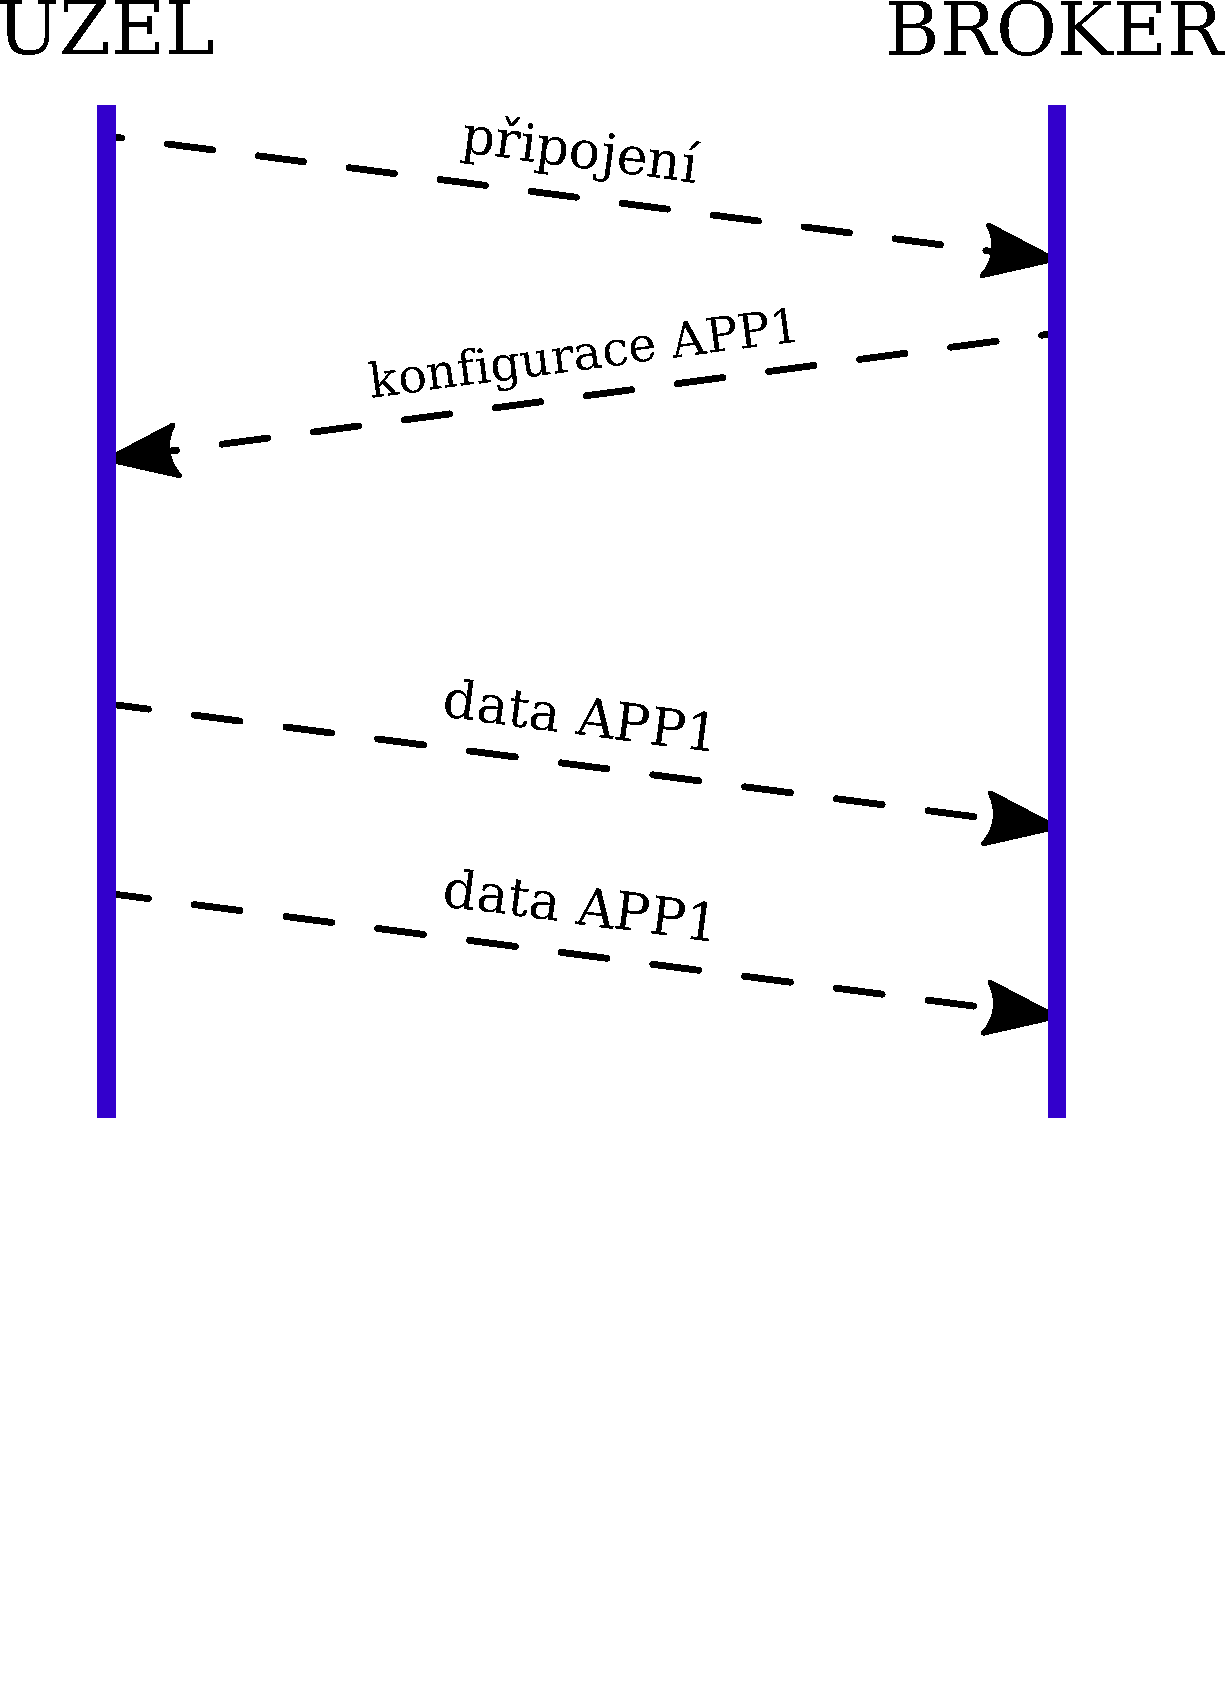
\includegraphics[width=.5\textwidth]{figures/messages-in-time.pdf}
    \caption{Diagram komunikace pomocí navrženého protokolu -- }
\end{figure}